\documentclass{article}
\usepackage{epsfig, latexsym}

\begin{document}

\newcommand{\bs}{\backslash}

\title{
\Huge{CMPEN 271 -- Fall 2012}\\
\normalsize{Exam 2}\\
\makebox[4in][l]{Name:} 
PSU ID:}
\date{}

\maketitle{}

\begin{tabular}{llll}
\begin{tabular}{c||c}
D & Q+   \\ \hline
0 & 0 \\ \hline
1 & 1 \\
\end{tabular}
&
\begin{tabular}{c||c}
T & Q+   \\ \hline
0 & Q \\ \hline
1 & Q' \\
\end{tabular}
&
\begin{tabular}{c|c||c}
S & R & Q+   \\ \hline
0 & 0 & Q \\ \hline
0 & 1 & 0 \\ \hline
1 & 0 & 1 \\ \hline
1 & 1 & x \\
\end{tabular}
&
\begin{tabular}{c|c||c}
J & K & Q+   \\ \hline
0 & 0 & Q \\ \hline
0 & 1 & 0 \\ \hline
1 & 0 & 1 \\ \hline
1 & 1 & Q' \\
\end{tabular}
\end{tabular}


\begin{enumerate}
\item {\bf (1 pt.)} Assuming a word size of 5 bits, interpret 11010 as a 2's complement
number.

\begin{tabular}{p{0.6in} p{0.6in} p{0.6in} p{0.6in} l}
a) -24 & b) -12 & c) -6 & d) -2 & e) None of the above.
\end{tabular}

\item {\bf (1 pt.)} Assuming a word size of 4 bits, determine the 2's complement
representation of -5.

\begin{tabular}{p{0.6in} p{0.6in} p{0.6in} p{0.6in} l}
a) 1011 & b) 1101 & c) 1100 & d) 1001 & e) None of the above.
\end{tabular}

\item {\bf (2 pt.)} How many AND gates are in a 4:16 decoder?

\begin{tabular}{p{0.6in} p{0.6in} p{0.6in} p{0.6in} l}
a) 4 & b) 8 & c) 16 & d) 32 & e) None of the above.
\end{tabular}


\item {\bf (2 pt.)} How many inputs do the AND gates in a 16:1 mux have?

\begin{tabular}{p{0.6in} p{0.6in} p{0.6in} p{0.6in} l}
a) 2 & b) 4 & c) 8 & d) 16 & e) None of the above.
\end{tabular}

\item {\bf (1 pt.)} How many 4:1 muxes are needed to construct a 8x4x1 mux?

\begin{tabular}{p{0.6in} p{0.6in} p{0.6in} p{0.6in} l}
a) 4 & b) 8 & c) 12 & d) 32 & e) None of the above.
\end{tabular}

\item {\bf (2 pt.)} How many 2:1 muxes are in an 8-bit register?

\begin{tabular}{p{0.6in} p{0.6in} p{0.6in} p{0.6in} l}
a) 2 & b) 3 & c) 4 & d) 8 & e) 64
\end{tabular}

\item {\bf (1 pt.)} How many address lines does a 256kx32 RAM have?

\begin{tabular}{p{0.6in} p{0.6in} p{0.6in} p{0.6in} l}
a) 32 & b) 19 & c) 18 & d) 16 & e) 15
\end{tabular}

\pagebreak
Questions 8-10 concern the construction of a bit-slice of a comparator.  The questions 
will ask you to complete the entries in the truth table below denoted by $a$, $b$, and
$c$.

\begin{tabular}{l|l|l|l|l||l|l|l}
$G_{in}$ & $L_{in}$ & $E_{in}$ & $x$ & $y$ & $G_{out}$ & $L_{out}$ & $E_{out}$ \\ \hline
    0    &    0     &     0    &  1  &  0  &   $a$     &           &           \\ \hline
    0    &    0     &     1    &  1  &  0  &           &   $b$     &           \\ \hline
    1    &    0     &     1    &  1  &  0  &           &           &    $c$    \\
\end{tabular}

\item {\bf (1 pt.)}What is the value of $a$?

\begin{tabular}{p{0.6in} p{0.6in} p{0.6in}}
a) 0 & b) 1 & c) x 
\end{tabular}

\item {\bf (1 pt.)}What is the value of $b$?

\begin{tabular}{p{0.6in} p{0.6in} p{0.6in}}
a) 0 & b) 1 & c) x 
\end{tabular}

\item {\bf (1 pt.)}What is the value of $c$?

\begin{tabular}{p{0.6in} p{0.6in} p{0.6in}}
a) 0 & b) 1 & c) x 
\end{tabular} \\

For questions 11-14 use the following figure

\scalebox{0.7}{\includegraphics{./Fig2/ExTim3}}

\item {\bf (1 pt.)} What is the value of Q1 at time 45

\begin{tabular}{p{0.75in}p{0.75in}p{1.75in}}
a) 0 & b) 1 & c) toggling \\
\end{tabular}

\item {\bf (1 pt.)} What is the value of Q1 at time 65

\begin{tabular}{p{0.75in}p{0.75in}p{1.75in}}
a) 0 & b) 1 & c) toggling \\
\end{tabular}

\item {\bf (1 pt.)} What is the value of Q2 at time 25

\begin{tabular}{p{0.75in}p{0.75in}p{1.75in}}
a) 0 & b) 1 & c) toggling \\
\end{tabular}

\item {\bf (1 pt.)} What is the value of Q2 at time 75

\begin{tabular}{p{0.75in}p{0.75in}p{1.75in}}
a) 0 & b) 1 & c) toggling \\
\end{tabular}

\pagebreak
You have a digital design which calls for a circuit which performs the 
following task (written as a C if/then statement).  You have decided on 
the architecture.  Its your job to design to complete the truth table
for the the glue-logic box (only an arbitrary portion of the complete 
truth table is shown).  I would recommend drawing a number line 
and putting the values of L6, L12, and L18 on it.  

\begin{verbatim}
if      (sum < 6)  z = sum
else if (sum < 12) z = sum-6
else if (sum < 18) z = sum-12
else               z = sum-18
\end{verbatim}

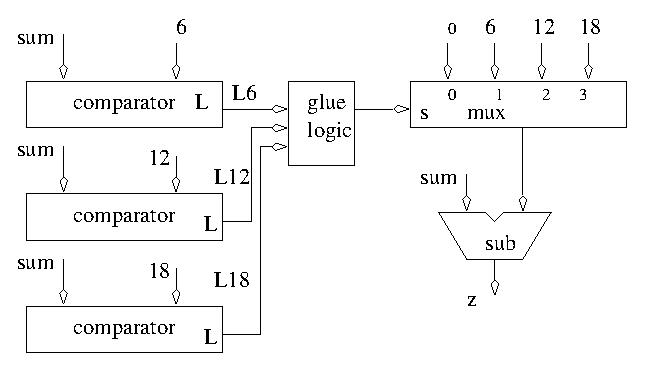
\includegraphics{./Fig2/if6}

\vspace{0.25in}

\begin{tabular}{l|l|l||l}
L6 & L12 & L18 & select \\ \hline
0  & 0   & 0   &   a   \\ \hline
0  & 1   & 1   &   b   \\ \hline
1  & 0   & 1   &   c   \\ 
\end{tabular}

\vspace{0.25in}

\item {\bf (1 pt.)}What is the (decimal) value of a in the truth table?

\begin{tabular}{p{0.6in} p{0.6in} p{0.6in} p{0.6in} l}
a) 0 & b) 1 & c) 2 & d) 3 & e) x  
\end{tabular}

\item {\bf (1 pt.)}What is the (decimal) value of b in the truth table?

\begin{tabular}{p{0.6in} p{0.6in} p{0.6in} p{0.6in} l}
a) 0 & b) 1 & c) 2 & d) 3 & e) x  
\end{tabular}

\item {\bf (1 pt.)}What is the (decimal) value of c in the truth table?

\begin{tabular}{p{0.6in} p{0.6in} p{0.6in} p{0.6in} l}
a) 0 & b) 1 & c) 2 & d) 3 & e) x  
\end{tabular}


\pagebreak

For questions 18,19 assume that a 4-bit (circular) shift register 
has the following truth table.   Complete the timing diagram below.

\begin{tabular}{l|l|l||l}
clk             & $C_1 C_0$     & D & $Q^+$  \\ \hline
0,1,$\downarrow$& xx            & x & Q      \\ \hline
$\uparrow$      & 00            & x & Q      \\  \hline
$\uparrow$      & 01            & x & $Q>>1$ (CSR) \\  \hline
$\uparrow$      & 10            & x & $Q<<1$ (CSL) \\  \hline
$\uparrow$      & 11            & D & D      \\
\end{tabular}

\scalebox{0.7}{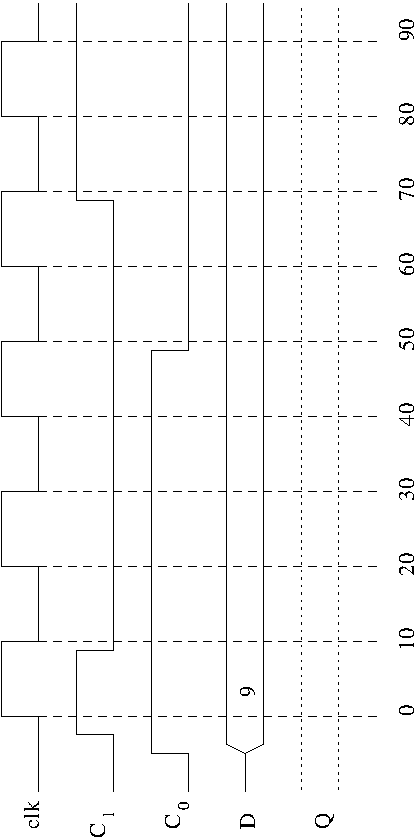
\includegraphics{./Fig2/shift-time2.eps}}

\item {\bf (1 pt.)}What is the value of $Q$ at time 55?

\begin{tabular}{p{0.6in} p{0.6in} p{0.6in} p{0.6in} l}
a) 0110 & b) 0010 & c) 0100 & d) 1110 & e) none of the above
\end{tabular}

\item {\bf (1 pt.)}What is the value of $Q$ at time 90?

\begin{tabular}{p{0.6in} p{0.6in} p{0.6in} p{0.6in} l}
a) 0001 & b) 1100 & c) 0100 & d) 1110 & e) none of the above
\end{tabular}

\item {\bf (2 pt.)} You have a digital design which calls for a circuit
which performs the following task.  You have decided on the architecture
shown to the right.  Its your job to design the contents of the glue-logic
box. Note, a register holds its value when the control input is 0 and 
loads its input when the control input is 1.

\begin{verbatim}
while (sum > 6) sum -= 6;
\end{verbatim}

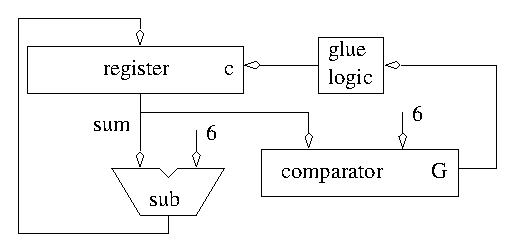
\includegraphics{./Fig2/while6}

\begin{tabular}{p{0.6in} p{0.6in} p{0.6in} p{0.6in} l}
a) c=0 & b) c=1 & c) c=G & d) c=G' & e) none of the above.  
\end{tabular}

\pagebreak
For problems 21-25 use the following figure and timing diagram.
You should assume that all the devices process 5-bits data 
values.

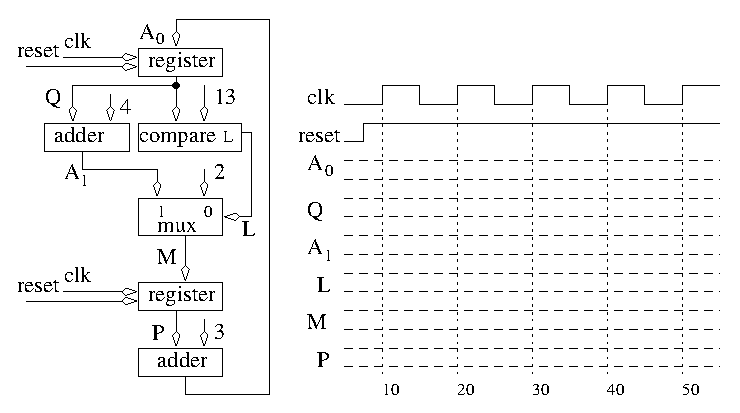
\includegraphics{./Fig2/BBBtiming3}

\item {\bf (2 pt.)}What is the value of $P$ at time 15?

\begin{tabular}{p{0.6in} p{0.6in} p{0.6in} p{0.6in} l}
a) 0  & b) 3  & c) 4  & d) 6  & e)  11
\end{tabular}

\item {\bf (2 pt.)}What is the value of $A_0$ at time 25?

\begin{tabular}{p{0.6in} p{0.6in} p{0.6in} p{0.6in} l}
a) 3  & b) 5  & c) 7  & d) 8 & e) 10
\end{tabular}

\item {\bf (1 pt.)}What is the value of $A_1$ at time 35?

\begin{tabular}{p{0.6in} p{0.6in} p{0.6in} p{0.6in} l}
a) 8  & b) 11  & c) 14 & d) 15  & e) 18
\end{tabular}

\item {\bf (1 pt.)}What is the value of $Q$ at time 45?

\begin{tabular}{p{0.6in} p{0.6in} p{0.6in} p{0.6in} l}
a) 5  & b) 7  & c) 11 & d) 13  & e) 14
\end{tabular}

\item {\bf (1 pt.)}What is the value of $M$ at time 55?

\begin{tabular}{p{0.6in} p{0.6in} p{0.6in} p{0.6in} l}
a) 2  & b) 5  & c) 7 & d) 8  & e) 9
\end{tabular}
\end{enumerate}
\end{document}
